We evaluate BibleGoAI across multiple dimensions: aggregate quality metrics, pipeline comparison, generation attempt analysis, and commentator tier contribution. All metrics are computed from the full corpus of generated BHTs: 7{,}957 New Testament verses and the full 39-book Old Testament, which is served via two complementary pipelines: a single-pass \emph{regular} pipeline (24 books, 10{,}492 verses) and a two-stage \emph{split} pipeline (20 books, 12{,}653 verses) whose two stages (\emph{split-a} and \emph{split-b}) are concatenated into a single served BHT per verse. The two pipelines overlap at the book level on 5 books (1~Kings, Esther, Habakkuk, Hosea, Micah) but cover different verses within them, so the comparison reported below is corpus-wide over each pipeline's own book set rather than a paired per-verse ablation.

\subsection{Aggregate Quality Metrics}

Table~\ref{tab:aggregate} summarizes the key metrics across the NT and OT corpora. The commentary-accuracy score (identical to what is exposed in legacy JSON outputs as \texttt{qualityScore}) is a composite tier-weighted similarity between the BHT and its source quotes; quote proportion measures the fraction of BHT words drawn directly from source commentary.

\begin{table}[htbp]
\centering
\footnotesize
\setlength{\tabcolsep}{3pt}
\caption{Aggregate BHT quality metrics across the three production sub-corpora: NT (single pipeline), OT regular (single-pass), and OT split (two-stage \emph{split-a}+\emph{split-b} concatenated per verse). The OT corpus as a whole spans 23{,}145 verses across all 39 books, partitioned by pipeline as shown. Commentary-accuracy and verse-accuracy scores for the split sub-corpus are per-verse means of the two stage scores; word count is the per-verse sum; quote proportion is word-count-weighted across the two stages. Values are mean $\pm$ standard deviation. Word counts are read from each BHT's stored \texttt{wordCount} field (computed by the pipeline's tokenizer at generation time); a re-computation by whitespace tokenization on the served text yields slightly lower values (e.g., 61.4 for OT regular and 83.2 for OT split-combined), reflecting tokenizer-vs-whitespace differences on contractions and punctuation.}
\label{tab:aggregate}
\begin{tabular}{@{}lccc@{}}
\toprule
 & \textbf{NT} & \textbf{OT reg.} & \textbf{OT split} \\
\textbf{Metric} & \textbf{(7{,}957)} & \textbf{(10{,}492)} & \textbf{(12{,}653)} \\
\midrule
Comm.\ Acc. & $1.91 \pm 0.35$ & $1.79 \pm 0.28$ & $1.82 \pm 0.25$ \\
Word Count & $84.2 \pm 11.1$ & $62.9 \pm 11.6$ & $85.9 \pm 13.5$ \\
Quote Prop.\ \% & $39.6 \pm 7.4$ & $31.8 \pm 6.3$ & $32.5 \pm 5.6$ \\
Verse Acc. & --- & $0.42 \pm 0.15$ & $0.41 \pm 0.14$ \\
\bottomrule
\end{tabular}
\end{table}

\noindent The NT corpus shows higher average commentary-accuracy scores than either OT sub-corpus (1.912 vs.\ 1.785 / 1.822), with longer BHTs than OT regular (84 vs.\ 63 words) and higher quote proportions (39.6\% vs.\ 31.8\% / 32.5\%). These differences are consistent with the structural contrast between the NT pipeline (verse-by-verse commentary, direct per-verse quote extraction) and the OT pipelines (multi-verse commentary, retrieval-augmented generation) described in Section~\ref{sec:methods}. The two OT sub-corpora produce comparable commentary-accuracy and verse-accuracy means despite their structural differences; the principal observable difference is length (the split sub-corpus's per-verse word count is roughly 1.4$\times$ that of OT regular because the served output is a concatenation of two stages). Verse accuracy was computed only for the OT corpus; see below for discussion.

\paragraph{A note on NT word count.} The observed NT mean (84.2 words) sits just above the target upper bound (80). The generation loop runs up to five attempts per verse and, if no candidate satisfies the full set of soft constraints (30--80 words, quote-proportion, etc.), the highest-scoring attempt is retained regardless of which constraints it misses. This best-of-five fallback prioritizes commentary quality over strict length compliance, yielding a mean that slightly overshoots the 80-word upper bound; see Section~\ref{sec:methods} for the full constraint-enforcement protocol.

\paragraph{Length and sentence-count compliance.} The Conciseness principle (Section~\ref{sec:introduction}) targets approximately 80 words and 2--4 sentences per BHT. Table~\ref{tab:length-compliance} reports realized statistics across the four generation variants in the corpus. NT generation consistently exceeded the 1--3 sentence prompt target (mean 4.2 sentences; 50.6\% of NT BHTs are exactly 4 sentences and 83.1\% exceed 3 sentences), while all three OT variants stayed within or below it. The split-pipeline served output (\emph{split-a} concatenated with \emph{split-b}) sums to roughly 3.3 sentences per verse on average, comparable to the regular OT pipeline's 2.7. The pattern parallels the word-count finding above: prompt-level length constraints were honored on OT but silently relaxed on NT, where the best-of-five quality-first selection appears to have favored slightly longer, multi-sentence outputs over strict constraint compliance.

\begin{table}[htbp]
\centering
\small
\setlength{\tabcolsep}{4pt}
\caption{Realized length and sentence-count statistics per generation variant, against a prompt-level target of approximately 80 words and 2--4 sentences (with an explicit 1--3 sentence soft target in the BHT prompts). Compliance is the percentage of BHTs in that variant landing in 1--3 sentences.}
\label{tab:length-compliance}
\begin{tabular}{@{}lrrrr@{}}
\toprule
\textbf{Variant} & $n$ & \textbf{Words} & \textbf{Sent.} & \textbf{1--3 sent.} \\
\midrule
NT v3 & 7{,}957 & 84.2 & 4.20 & 16.9\% \\
OT regular & 10{,}492 & 62.9 & 2.74 & 94.3\% \\
OT split-a & 12{,}653 & 55.1 & 2.33 & 98.5\% \\
OT split-b & 12{,}653 & 30.8 & 1.00 & 100.0\% \\
\bottomrule
\end{tabular}
\end{table}

\paragraph{Verse accuracy (OT only).}
\label{sec:verse-acc}
The \emph{verse accuracy} metric (cosine similarity between the BHT and the target-verse embedding) was computed only for the OT corpus ($0.417 \pm 0.147$). The metric is not meaningful for the NT pipeline because NT BHTs are produced from per-verse commentary directly tied to the target verse; it exists specifically as a sanity check on the OT RAG pipeline, which must select the right span across multi-verse commentary.

\subsection{Pipeline Comparison: Regular vs.\ Split}
\label{sec:strategy}

Two OT generation pipelines were built, each run once over a different subset of the OT canon:

\begin{itemize}[nosep,leftmargin=*]
    \item \textbf{Regular pipeline}: A single-pass generation that produces one BHT per verse from tagged commentary, targeting 30--80 words. Run over 24 OT books (10{,}492 verses), predominantly wisdom, prophetic, and selected historical books where per-verse commentary coverage was adequate.
    \item \textbf{Split pipeline}: A two-stage generation where \emph{split-a} produces a short factual paragraph and \emph{split-b} adds one enriching sentence; the two outputs are concatenated per-verse into a single BHT, with a combined score computed as the mean of the two stage scores. Run over 20 OT books (12{,}653 verses), predominantly Pentateuch and historical narrative where verse-range commentary dominates and the split was developed to handle broader context.
\end{itemize}

\paragraph{A note on the comparison.} The two pipelines were developed sequentially and run over mostly disjoint book sets. Five books (1~Kings, Esther, Habakkuk, Hosea, Micah) appear in both pipelines' outputs, but inspection reveals that the two pipelines covered \emph{different chapters} of these books with no overlapping verses---the regular-pipeline outputs for these books are experimental partial runs that never reached production. As a result, no paired per-verse head-to-head comparison is possible from the generated corpus; Table~\ref{tab:strategy} reports corpus-wide means over each pipeline's own book set.

\begin{table}[htbp]
\centering
\small
\caption{Pipeline comparison across the OT corpus. Numbers are corpus-wide means over each pipeline's own book set (regular: 24 books; split: 20 books); the two sets overlap at the book level on 5 books but the regular-pipeline outputs for those books are partial experimental runs covering different verses than the split-pipeline outputs, so a paired per-verse comparison is not possible.}
\label{tab:strategy}
\begin{tabular}{@{}lcc@{}}
\toprule
\textbf{Metric} & \textbf{Regular} & \textbf{Split (combined)} \\
\midrule
$n$ (verses) & 10{,}492 & 12{,}653 \\
$n$ (books) & 24 & 20 \\
Commentary Accuracy & 1.785 & 1.822 \\
Word Count & 62.9 & 85.9 \\
Quote Prop.\ (\%) & 31.8 & 32.5 \\
\bottomrule
\end{tabular}
\end{table}

\noindent The two pipelines produce BHTs with comparable commentary-accuracy means (1.78 vs.\ 1.82) and near-identical quote-token proportions (${\sim}32\%$), indicating comparable source-fidelity behavior; Figure~\ref{fig:strategy} visualizes the same comparison. The main observable difference is length: split-pipeline BHTs are roughly 37\% longer (86 vs.\ 63 words) because the concatenation of \emph{split-a} and \emph{split-b} yields a two-paragraph output. Because the two pipelines cover different book sets, these corpus-wide means should be read as per-pipeline performance characteristics on the books each was actually run over---not as a controlled ablation.

\paragraph{Stage-level view (split pipeline only).} Within the split pipeline, \emph{split-a} produces longer, higher-scoring paragraphs on its own (mean commentary-accuracy 1.935, mean word count 55.1) while \emph{split-b} produces shorter, lower-scoring enriching sentences (mean 1.710, mean word count 30.8). These are not alternative strategies (both stages always run together, and the combined served BHT is their concatenation), but the per-stage numbers illustrate the intended asymmetric roles of the two sub-prompts.

\begin{figure}[t]
\centering
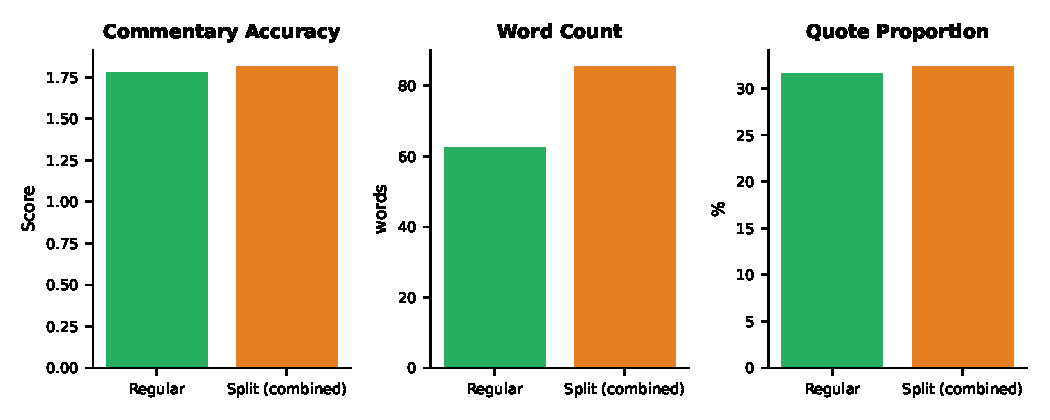
\includegraphics[width=0.95\columnwidth]{figures/strategy_comparison.pdf}
\caption{Corpus-wide means for the Regular and Split (combined) OT pipelines across each pipeline's own book set.}
\label{fig:strategy}
\end{figure}

\subsection{Generation Attempt Analysis}

The system generates up to five candidate BHTs per verse and selects the highest-scoring attempt. Figure~\ref{fig:attempts} shows the average commentary-accuracy score at each attempt number across all NT and OT runs combined ($n{=}43{,}755$ first attempts), which reveals a counter-intuitive pattern: mean scores \emph{decrease} monotonically with attempt index (1.74, 1.70, 1.69, 1.68, 1.67 for attempts 1 through 5). This is not evidence that later generations are worse in absolute terms; rather, it reflects the selection dynamics of the loop: later attempts are only triggered when earlier attempts fail the hard constraint gate (word count, quote proportion, forbidden tokens), so attempts 2--5 are drawn from a harder subset of verses where the generator has already struggled. The best-of-five selection then routinely picks the first-attempt BHT. In the production run, the majority of verses succeeded on attempt~1, and the retry budget primarily functioned as safety capacity for the minority of verses where the first attempt tripped a hard constraint.

\begin{figure}[t]
\centering
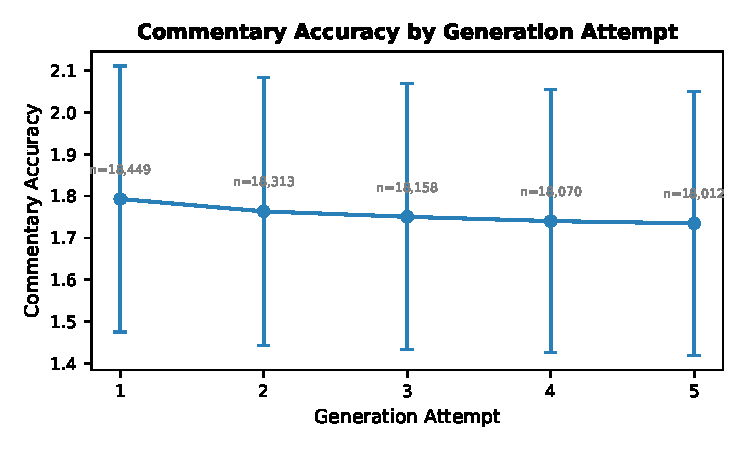
\includegraphics[width=0.95\columnwidth]{figures/attempt_trajectory.pdf}
\caption{Mean commentary-accuracy score at each generation attempt (1--5). Scores decrease with attempt index because later attempts are only triggered when earlier ones fail the hard constraint gate, so attempts 2--5 are drawn from a harder subset of verses.}
\label{fig:attempts}
\end{figure}

\subsection{Commentator Tier Contribution}

Figure~\ref{fig:tiers} shows the distribution of tier-weighted semantic similarity across the three commentator tiers, expressed as the percentage of each tier's contribution to the final BHT's similarity profile (values sum to 100\% per verse, averaged across the corpus). The NT corpus shows a flatter distribution than the prompt's ``primarily Tier~1, sparingly Tier~2, minimally Tier~3'' instruction would suggest: NT Tier~1 31.8\%, Tier~2 31.2\%, Tier~3 37.0\%. The full per-verse OT corpus follows the prompt ordering more cleanly (Tier~1 41.8\%, Tier~2 34.0\%, Tier~3 24.1\%) but is heavily influenced by the split pipeline's \emph{split-b} stage, which intentionally uses no Tier~3 commentators (Tier~3 contribution is zero by construction in split-b). For comparison, the OT regular sub-corpus alone yields Tier~1 35.1\%, Tier~2 29.7\%, Tier~3 35.1\%---a flatter distribution similar to NT. The NT result indicates the tier instruction is not strongly followed in the produced output. One likely cause is that several Tier~3 commentators produce longer and more thematically broad excerpts than the Tier~1 commentators, yielding higher surface-level similarity scores even when they contribute less content by intent. Reconciling the intent-based tiering with similarity-based measurement is a natural follow-up for future tuning.

\begin{figure}[t]
\centering
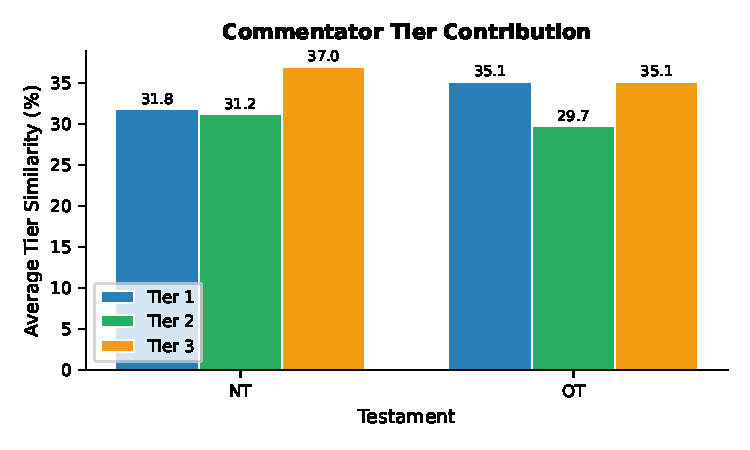
\includegraphics[width=0.95\columnwidth]{figures/tier_breakdown.pdf}
\caption{Average commentator-tier contribution to BHT semantic similarity, as a percentage summing to 100\% per verse. NT shows a flat distribution where Tier~3 contributes at or above the level of Tier~1, indicating that the tier instruction is not strongly followed. The OT per-verse curve appears to follow the prompt ordering more cleanly, but this is driven by the split pipeline's \emph{split-b} stage, which intentionally uses no Tier~3 commentators by construction.}
\label{fig:tiers}
\end{figure}

\subsection{Commentary-Accuracy Score Distribution}

Figure~\ref{fig:quality_dist} presents the distribution of commentary-accuracy scores across the NT and OT corpora. Both distributions are approximately Gaussian with a right-skew tail toward higher-scoring verses. For the NT corpus ($n{=}7{,}957$), the 5th, 25th, 50th, 75th, and 95th percentiles are 1.32, 1.68, 1.93, 2.14, and 2.46 respectively. The full per-verse OT corpus ($n{=}23{,}145$, with split-pipeline verses scored as the mean of their \emph{split-a} and \emph{split-b} stages) runs slightly lower: 1.37, 1.62, 1.80, 1.98, and 2.25 at the same percentiles. The retry-loop stopping threshold is a score of 2.3 (Section~\ref{sec:scoring}), which sits near the 85th percentile of NT scores and above the 95th percentile of OT per-verse scores. This threshold governs when generation stops, not which BHTs are retained: if no attempt ever clears~2.3, the best-scoring attempt is still kept (best-of-five fallback) to avoid coverage gaps, so a meaningful minority of retained BHTs fall below~2.3. A separate display-time cutoff on BibleGo.org (Section~\ref{sec:scoring}) hides very-low-scoring BHTs from readers while keeping them in the served corpus.

\begin{figure}[t]
\centering
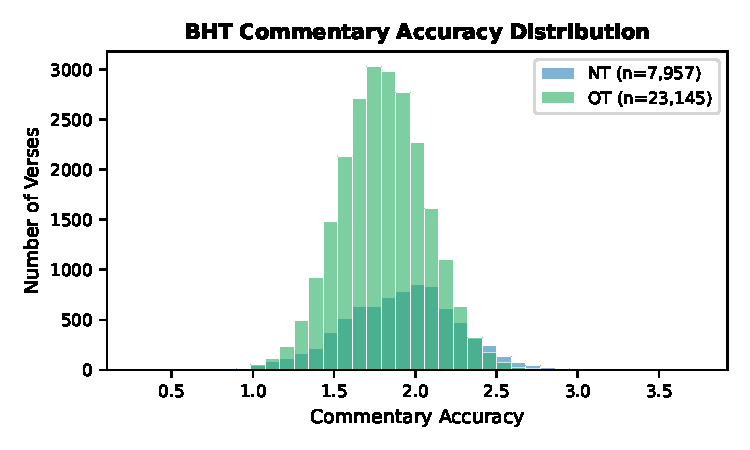
\includegraphics[width=0.95\columnwidth]{figures/quality_distribution.pdf}
\caption{Distribution of commentary-accuracy scores across the NT ($n{=}7{,}957$) and OT per-verse ($n{=}23{,}145$, split-pipeline verses scored as the mean of their two stages) corpora. Both distributions are approximately Gaussian with a right-skew tail; the nominal acceptance threshold (2.3) sits near the 85th percentile of NT scores and above the 95th percentile of OT per-verse scores.}
\label{fig:quality_dist}
\end{figure}

\subsection{Human Evaluation}

In addition to automated metrics, BHT quality was evaluated through two rounds of structured user testing with members of the project's Bible study community:

\begin{itemize}[nosep,leftmargin=*]
    \item \textbf{BHT V2 Quality Test}: Human raters scored NT BHTs on a normalized quality scale. Scores ranged from 50.4 to 94.2 out of 100, with a mean of 67.5. The highest-rated BHT (Romans 6:7, score 94.2) demonstrated strong synthesis of commentary insights, while lower-scoring BHTs guided subsequent prompt refinements.
    \item \textbf{OT BHT V1 Quality Test}: A separate round evaluated the first generation of OT BHTs, providing feedback that informed the comparison of RAG versus tagging strategies.
\end{itemize}

\noindent Table~\ref{tab:human} presents the human quality scores from the BHT V2 evaluation. Note that these are a separate metric from the automated \emph{commentary-accuracy} score discussed above: raters scored each BHT on a normalized 0--100 quality scale.

\begin{table}[htbp]
\centering
\small
\caption{Human evaluation scores (BHT V2 Quality Test). Human-assigned 0--100 quality ratings; distinct from the automated commentary-accuracy score in Table~\ref{tab:aggregate}.}
\label{tab:human}
\begin{tabular}{@{}lc@{}}
\toprule
\textbf{Verse} & \textbf{Human Score} \\
\midrule
Romans 6:7 & 94.2 \\
John 5:22 & 80.1 \\
Ephesians 1:22 & 77.3 \\
Ephesians 6:13 & 65.5 \\
Galatians 5:22 & 62.7 \\
John 10:27 & 57.0 \\
Romans 6:21 & 54.1 \\
Revelation 3:3 & 50.4 \\
\midrule
\textbf{Mean} & \textbf{67.7} \\
\bottomrule
\end{tabular}
\end{table}

\noindent These human scores, combined with the automated quality metrics, provided a feedback loop that drove iterative prompt refinement: most notably the May 2024 prompt updates that shifted the choicest extraction focus from ``striking and enlightening'' to ``helpful, explanatory, and illuminating'' quotes targeting basic words and facts in each verse.
